\section{Introduction}\label{sec:introduction}

In this project students were asked to implement, using the knowledge acquired from lectures and the AIMA book reading, the air cargo problem using first order logic. Students had also to implement functions of the \textsc{Graphplan} algorithm, this time using the techniques from the AIMA book.

In this report, the experimental results from search a solution in problems 1, 2 and 3 using different techniques will be available in sections \ref{sec:p1_results}, \ref{sec:p2_results} and \ref{sec:p3_results} respectively. A discussion of these results, based on the knowledge leveraged so far, is presented in section \ref{sec:conclusion}.

\section{Problem 1 Results}\label{sec:p1_results}

With only 2 fluents in its goal set and 20 in the actions list, the problem did not take much time to solve, as shown in the graphs. The optimal solution for the problem is shown bellow, followed by some charts to facilitate data visualization.

\begin{flushleft}
	Optimal solution:
	\begin{itemize}
		\item \textit{Load(C1, P1, SFO)}
		\item \textit{Load(C2, P2, JFK)}
		\item \textit{Fly(P1, SFO, JFK)}
		\item \textit{Fly(P2, JFK, SFO)}
		\item \textit{Unload(C1, P1, JFK)}
		\item \textit{Unload(C2, P2, SFO)}
	\end{itemize}
\end{flushleft}

\begin{figure}[ht]
	\centering
	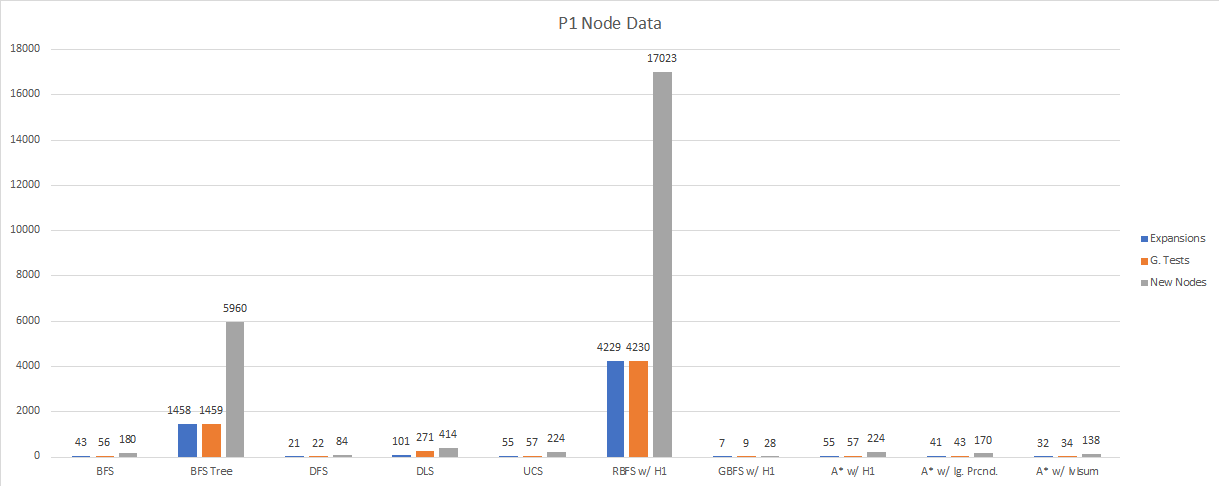
\includegraphics[width=0.9\textwidth]{images/P1_node_data.png}
	\caption{Problem 1: expansions, goal tests and new nodes}
	\label{fig:p1_node_data}
\end{figure}

\begin{figure}[ht]
	\centering
	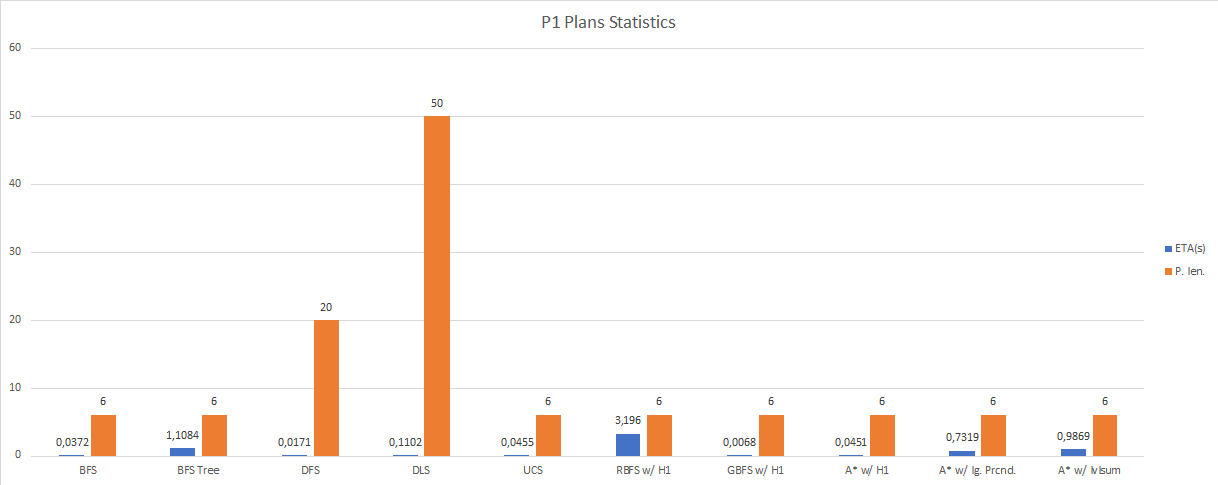
\includegraphics[width=0.9\textwidth]{images/P1_plan_statistics.png}
	\caption{Problem 1: ETA in seconds and solution length}
	\label{fig:p1_plan_statistics}
\end{figure}

\section{Problem 2 Results}\label{sec:p2_results}

As expected, in general, problem 2 took longer to solve than problem 1, due to its 3 fluents goal and 72 fluents in the action list. In fact, using the Bread First Tree Search and Recursive Best First Tree Search was infeasible to solve this problem, due to its long time to process. An optimal solution is presented bellow followed by 2 charts similar to the ones found in section \ref{sec:p1_results}.

\begin{flushleft}
	Optimal solution:
	\begin{itemize}
		\item \textit{Load(C1, P1, SFO)}
		\item \textit{Load(C2, P2, JFK)}
		\item \textit{Load(C3, P3, ATL)}
		\item \textit{Fly(P1, SFO, JFK)}
		\item \textit{Fly(P2, JFK, SFO)}
		\item \textit{Fly(P3, ATL, SFO)}
		\item \textit{Unload(C1, P1, JFK)}
		\item \textit{Unload(C2, P2, SFO)}
		\item \textit{Unload(C3, P3, SFO)}
	\end{itemize}
\end{flushleft}

\begin{figure}[ht]
	\centering
	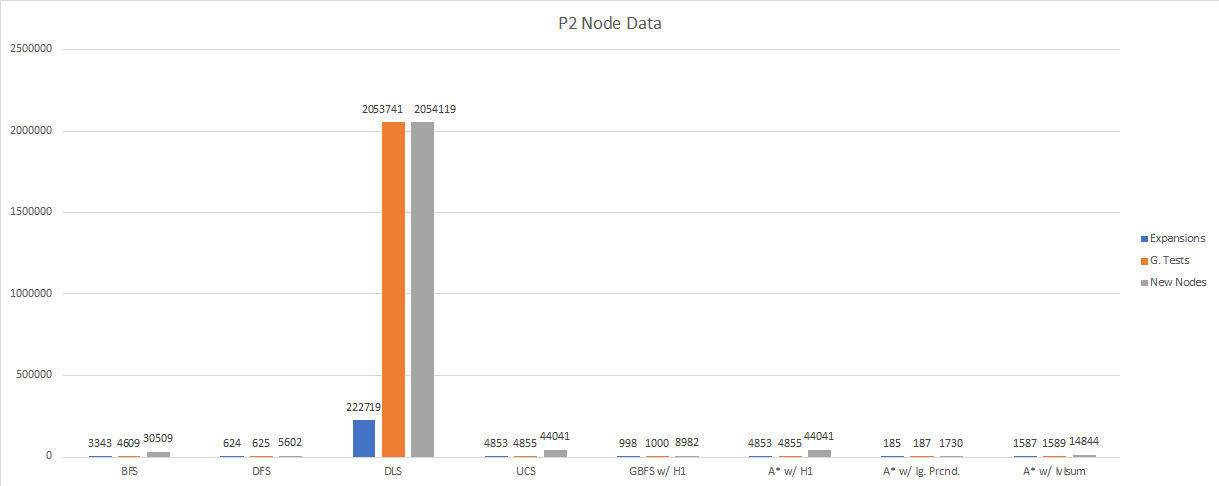
\includegraphics[width=0.9\textwidth]{images/P2_node_data.png}
	\caption{Problem 2: expansions, goal tests and new nodes}
	\label{fig:p2_node_data}
\end{figure}

\begin{figure}[ht]
	\centering
	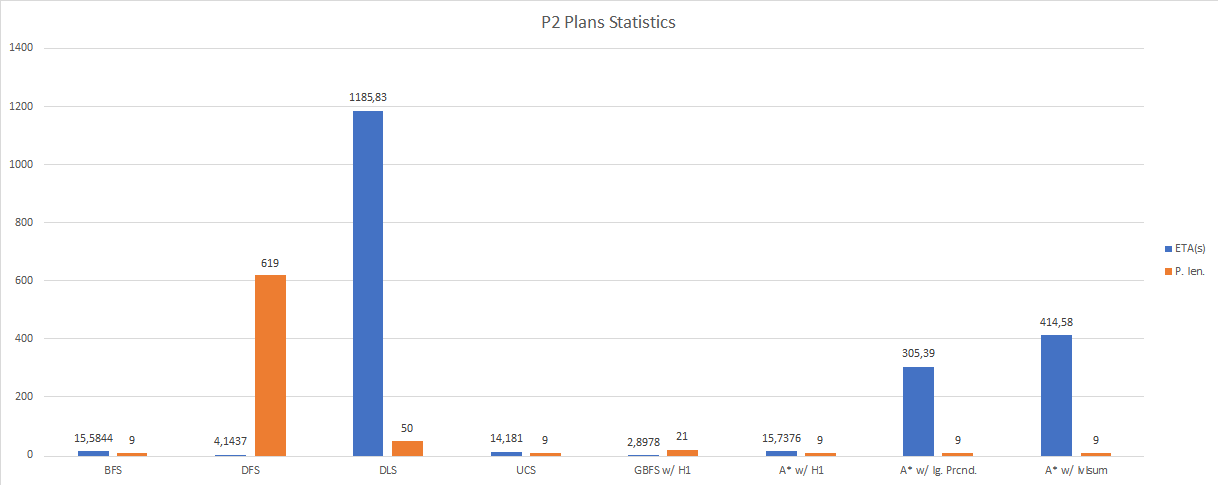
\includegraphics[width=0.9\textwidth]{images/P2_plan_statistics.png}
	\caption{Problem 2: ETA in seconds and solution length}
	\label{fig:p2_plan_statistics}
\end{figure}

\section{Problem 3 Results}\label{sec:p3_results}

This problem adds 1 more fluent to the goal compared to problem 2, and its action list has 88 available actions, making it harder to solve than problem 1 and 2. As expected it did take longer to solve, and one more search algorithm, Depth-Limited Search, was unable to solve the problem in a feasible time, at least to my constraints. The optimal solution is presented bellow followed by the result charts.

\begin{flushleft}
	Optimal solution:
	\begin{itemize}
		\item \textit{Load(C1, P1, SFO)}
		\item \textit{Load(C2, P2, JFK)}
		\item \textit{Fly(P1, SFO, ATL)}
		\item \textit{Fly(P2, JFK, ORD)}
		\item \textit{Load(C3, P1, ATL)}
		\item \textit{Load(C4, P2, ORD)}
		\item \textit{Fly(P1, ATL, JFK)}
		\item \textit{Fly(P2, ORD, SFO)}
		\item \textit{Unload(C1, P1, JFK)}
		\item \textit{Unload(C3, P1, JFK)}
		\item \textit{Unload(C2, P2, SFO)}
		\item \textit{Unload(C4, P2, SFO)}
	\end{itemize}
\end{flushleft}

\begin{figure}[ht]
	\centering
	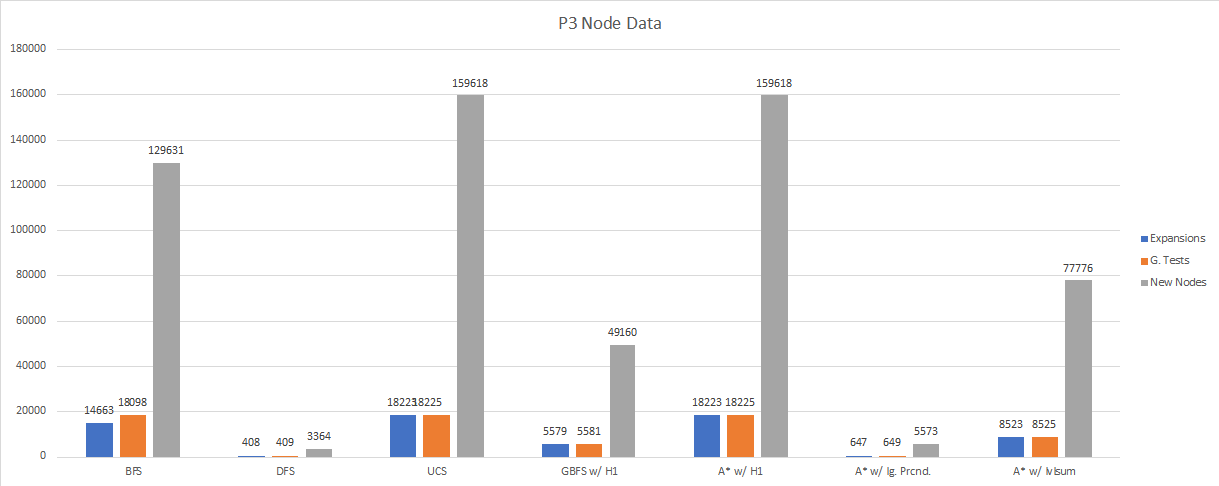
\includegraphics[width=0.9\textwidth]{images/P3_node_data.png}
	\caption{Problem 3: expansions, goal tests and new nodes}
	\label{fig:p3_node_data}
\end{figure}

\begin{figure}[ht]
	\centering
	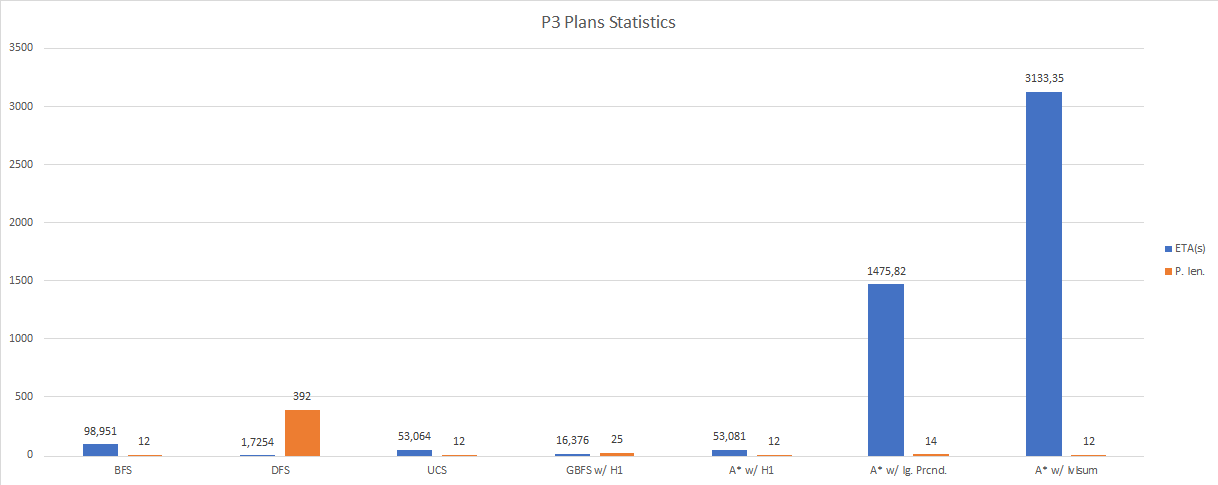
\includegraphics[width=0.9\textwidth]{images/P3_plan_statistics.png}
	\caption{Problem 3: ETA in seconds and solution length}
	\label{fig:p3_plan_statistics}
\end{figure}


\section{Conclusion}\label{sec:conclusion}

In the lectures and in \cite{aima}, various search algorithms have been presented, one of them is the Breadth First Search which takes shortest, i.e. the path with the least number of nodes, to be analyzed. This path is guaranteed to find the shortest path as can be seen in all the charts, in all 3 problems it did found a solution with the minimum number of fluents.

Another search algorithm used is the Depth First Search, this algorithm is not guaranteed to find an optimal solution because it goes deep in the search space until it finds a leaf, but if the tree is infinite, it’s not even guaranteed to find a solution. Due to the structure of the planning graph, this algorithm was able to find a plan quickly, but as shown in the charts, the number of fluents in the plans is almost equal to the number of expanded nodes. If the problem 1 had thousands of airports instead of just 2, the length of the plan could also have thousands of actions more, thus making this algorithm not suited to solve this kind of problem. 

The Uniform Cost Search is quite similar to the DFS algorithm, but instead of deciding on the path length to expand a path, this one analyses the cost of the path. With that being said, this algorithm is guaranteed to find a solution with the minimal cost, and after performing the tests, the plans returned by this function were equal to the ones provided as optimal solutions in section 2 through 4. Because this function analyses the path cost and not the path length, it doesn't backtrack as much as the DFS, since a longer path can continue to be expanded instead of the shorter path, due to the lesser cost of the longer path.

Finally, the A* algorithm combines the path cost of the UCS and a heuristic function to provide some informed guidance to the agent, more or less like an educated guess. In the project three heuristics have been used: H1, Ignore Preconditions and Level Sum, and as these functions are admissible, then the A* search could find the least cost path. Observing the charts, all three functions almost always returned a path with the same length, the biggest differences in these functions were the number of expanded nodes and ETA to solve the problems. The first function, H1, is the simplest one, being fast to compute but also being further from the real value, in the tests this function have been the fastest of the 3 because of its simplicity, but also the one that expanded the most number nodes. The second one, Ignore Preconditions, gave excellent guidance with the least number of expanded nodes, but because of its higher complexity, it did take longer to complete. The Level Sum provides better guidance than the H1, as can be seen by the smaller number of expanded nodes, but as it is more complex to compute, the agent also took longer to find a solution.

